\documentclass[letterpaper, 10 pt, conference]{ieeeconf}
\let\labelindent\relax% Comment this line out if you need a4paper

%\documentclass[a4paper, 10pt, conference]{ieeeconf}      % Use this line for a4 paper

\IEEEoverridecommandlockouts                              % This command is only needed if 
                                                          % you want to use the \thanks command

\overrideIEEEmargins
% The preceding line is only needed to identify funding in the first footnote. If that is unneeded, please comment it out.
\usepackage{booktabs}
\usepackage{amsmath}
\usepackage{balance}
\usepackage{enumitem}
% \usepackage{amsthm}
\usepackage{hyperref}
\usepackage{amssymb}
\usepackage{colortbl}
\usepackage{stfloats}
\usepackage{xcolor} 
\usepackage{textcomp}
\usepackage{graphicx}
\usepackage{verbatim}
\usepackage{multirow}
\usepackage{algorithm}
\usepackage{multicol}
\usepackage{algpseudocode}
\usepackage{mathtools}
\newtheorem{theorem}{Theorem}
\newtheorem{lemma}[theorem]{Lemma}
\newtheorem{definition}{Definition}
\usepackage{hyperref}
\usepackage{subcaption}





\graphicspath{{./pdf/}{./jpeg/}{./eps/}}

\algrenewcommand\algorithmicrequire{\textbf{Input:}}
\algrenewcommand\algorithmicensure{\textbf{Output:}}
\def\BibTeX{{\rm B\kern-.05em{\sc i\kern-.025em b}\kern-.08em
    T\kern-.1667em\lower.7ex\hbox{E}\kern-.125emX}}




\title{\LARGE \bf
Quantum Approaches for Dysphonia Assessment \\in Small Speech Datasets 
}


\author{Ha Tran$^{1}$, Bipasha Kashyap$^{1}$, \textit{Member, IEEE}, Pubudu N. Pathirana$^{1}$, \textit{Senior Member, IEEE}% <-this % stops a space
\thanks{$^{1}$All authors are with the Networked Sensing \& Biomedical Engineering (NSBE) Research lab, School of Engineering, Deakin University, Waurn Ponds, Victoria, AU.
        {\tt\small thi.n.tran@deakin.edu.au, aubipasha@deakin.edu.au, pubudu@deakin.edu.au}}%
}


\begin{document}



\maketitle
\thispagestyle{empty}
\pagestyle{empty}


%%%%%%%%%%%%%%%%%%%%%%%%%%%%%%%%%%%%%%%%%%%%%%%%%%%%%%%%%%%%%%%%%%%%
\begin{abstract}
Dysphonia, a prevalent medical condition, leads to voice loss, hoarseness, or speech interruptions. To assess it, researchers have been investigating various machine learning techniques alongside traditional medical assessments. Convolutional Neural Networks (CNNs) have gained popularity for their success in audio classification and speech recognition. However, the limited availability of speech data, poses a challenge for CNNs. This study evaluates the performance of CNNs against a novel hybrid quantum-classical approach, Quanvolutional Neural Networks (QNNs), which are well-suited for small datasets. The audio data was preprocessed into Mel spectrograms, comprising 243 training samples and 61 testing samples in total, and used in ten experiments. Four models were developed (two QNNs and two CNNs) with the second models incorporating additional layers to boost performance.
The results revealed that QNN models consistently outperformed CNN models in accuracy and stability across most experiments.

\indent \textit{Clinical relevance}— This work investigates the potential of quantum-based approaches for medical data classification and their promising role in enhancing dysphonia assessment.
\end{abstract}

\section{Introduction}
Speech is a fundamental aspect of human communication, facilitated by the coordinated function of various organs. However, these organs can be compromised by neurological disorders such as Parkinson’s, Ataxia, and Dysphonia, making communication challenging for many individuals. Dysphonia, a prevalent medical condition, affects approximately 10\% of the general population and 50\% of professional voice users~\cite{martins2016voice}. Those who use their voice extensively, such as teachers, or individuals in older age groups, are more prone to developing this condition. Symptoms of Dysphonia often include hoarseness, a weak or breathy voice, strained speech, or even voice loss, typically caused by malformations or dysfunctions of the vocal cords or the larynx (voice box).  

Dysphonia can be assessed by medical history, symptom assessment, and laboratory examination. Assessment can be done using the GRBAS (Grade, Roughness, Breathiness, Asthenia, and Strain) scale to assess voice quality ~\cite{hirano1981clinical}. Equipment such as a laryngoscope is used to examine the vocal cords and larynx. Imaging tests such as CT or MRI scans can be used to recognize structural or neurological abnormalities. However, these methods are time-consuming, discomfort for patients, and expensive. According to~\cite{cohen2012direct}, a patient needs to pay from 577 to 953 US dollars per year for diagnosing and managing the disorder.    

Machine learning has made significant advancements in analysing voice signals, which can be effectively used to assess dysphonia and other voice disorders. Some common features of voice signals such as Mel-Frequency Cepstral Coefficients (MFCCs), jitter, and shimmer are extracted as the input of models such as Random Forest, Decision Trees, Support Vector Machine (SVM), Gaussian Mixture Model Supervector Kernel-support Vector Machine (GMM-SVM)~\cite{verde2018voice, rehman2024voice, dankovivcova2018machine, wang2011discrimination}. Although these works achieved high accuracy in detecting Dysphonia, these ML algorithms require expertise and experience in feature selection and combination.  

Deep learning methods, such as Convolutional Neural Networks (CNNs), have been widely used in tasks like image recognition, speech classification, and natural language processing. These methods have also shown promise in assessing pathological speech by leveraging advanced feature extraction and classification capabilities. Specifically, in~\cite{islam2022voice}, CNN was used to classify the Dysphonia and normal voices and achieved an accuracy of 82.33\%. The study~\cite{wu2018convolutional}  achieved 88.5\%, 66.2\%, and 77\% classification accuracy on training, validation, and testing data using CNN. Despite these promising results, the application of deep neural networks to speech-related rare disorders is challenging due to the limited availability of medical data. Small datasets often result from the rarity of these conditions, and hospitals are often hesitant to share data due to privacy concerns. To address these challenges, researchers have explored techniques like oversampling, as demonstrated in ~\cite{lee2023efficient}, where CNNs with oversampling achieved an impressive accuracy of 98.9\%. Another approach ~\cite{peng2023voice} utilized a combination of pre-trained CNNs and SVM classifiers to enhance performance with limited data, using Mel spectrograms as input. The study~\cite{chen2023deep} divided audio files to augment the data and used CNN to classify Dysphonia and normal people based on MFCCs, and Mel spectrogram features. This framework obtained 92\% accuracy, 98\% recall, 89\% precision, and 87\% specificity. These advancements highlight the potential of deep learning in speech pathology but underscore the need for innovative solutions to overcome data scarcity and privacy barriers.


In recent years, quantum machine learning~\cite{schuld2021machine} has been an emerging field with various applications. Classical machine learning algorithms still suffer from computational bottlenecks such as model complexity, high dimensionality, and processing power. Some researchers show that quantum algorithms can perform well on small datasets. In~\cite{sagheer2019novel}, an autonomous perceptron model (APM) inspired by the computational power of the qubit outperformed some classical machine learning models in terms of accuracy and computational time with the limited number of training samples. In~\cite{acar2021covid}, quantum transfer learning was used to detect COVID-19 from CT images and achieved an accuracy of 90\% to 100\% using 20\% and 80\% of training and testing data. Relatively little study has been done in the field of quantum speech thus far.~\cite{qi2022classical} proposes a hybrid transfer learning approach combining classical CNN and Variational Quantum Circuit (VQC)-based Quantum Neural Network to enhance spoken command recognition on noisy intermediate-scale quantum (NISQ) devices, achieving improved performance on the Google Speech Commands dataset. ~\cite{hong2022qspeech} proposed a Quantum Neural Network with a low-qubit VQC and created a comprehensive application framework known as QSpeech. ~\cite{chen2024consensus} introduces a Consensus-based Distributed Quantum Kernel Learning (CDQKL) framework designed to enhance speech recognition by distributing computational tasks across quantum terminals connected via classical channels, thereby preserving data privacy and improving scalability.   In 2021,~\cite{yang2021decentralizing} proposed a distributed speech command recognition algorithm based on a Quantum Convolutional Neural Network (QCNN) or QNN, encoding Mel spectrograms of audio by using 2 × 2 quantum convolution layers, with subsequent networks being classical deep learning networks. The experiment results showed that the algorithm achieved an accuracy of 95.12\% on the Google Speech Commands dataset. 


As per our literature review, there is currently no prior work on the benefits of Quantum approaches in detecting voice and speech disorders. This study is a novel attempt at hybrid quantum-classical algorithms, the Quanvolutional Neural Network (QNN)~\cite{henderson2020quanvolutional}, which combines the advantages of quantum and classical technology, to detect Dysphonia. The contributions of this paper are as follows.

1. Investigating the behaviour of the hybrid quantum model in detecting voice disorder.

2. Comparing experimental results and analysing the performances between CNNs and QNNs on small datasets.
\section{Methodology}
\label{method}
\subsection{Processing Speech}
\label{subsection: speech process}
A Mel spectrogram is a visual representation of frequencies over time of the audio signal. It is one of the common features used in fields such as speech recognition~\cite{park2019specaugment}, audio classification~\cite{xu2018large, meghanani2021exploration}. Figure~\ref{fig:speech process} shows the process of converting an audio signal into a Mel spectrogram. Specifically, the audio time-domain signal is divided into overlapping frames using a windowing function such as a Hamming or Hann window. Each frame is then transformed into a spectrogram representing frequencies over time using the Fourier Transform. The spectrogram is passed through a Mel filter bank and converted to a logarithmic scale in decibels (dB). The final output is a 2D Mel spectrogram image, where the time and frequency are on the horizontal and vertical axis. In this study, the Mel spectrogram is generated using the Librosa library with a window size of 2048, hop-length of 512 samples, 2048-point Fast Fourier Transform, 128 Mel bands, and Grayscale intensity to reduce the complexity. The final Mel spectrogram having the dimension of 40-by-100-by-1 (height-by-weight-by-channel) is used as the input of the QNNs below.

\begin{figure}[htbp]
    \centering
    \includegraphics[width=0.5\textwidth]{Speech_process.drawio.pdf}
    \caption{The speech processing.}
    \vspace{-10pt}
    \label{fig:speech process}
\end{figure}

\subsection{Quanvolutional Neural Network}
QNN is the hybrid quantum-classical neural network. The quanvolutional layer replaces the convolutional layer in the classical CNN model to improve performance by extracting features using quantum circuit properties. These features are subsequently aggregated and passed to the following layers in the classical neural network, enabling further processing and classification.


\subsubsection{\textbf{Quanvolutional Layer}}
\label{subsub:Quanv layer}
A quanvolutional layer, which contains many quanvolutional filters, transforms patches of the input tensor using quantum circuits instead of performing element-wise matrix multiplication like the classical convolutional layer. These circuits, which can be structured or random, process the data by utilizing quantum properties such as superposition and entanglement. In this study, we use a 2-by-2 quanvolutional filter, corresponding to four qubits and a random quantum circuit. Figure~\ref{fig:Quanvolutional layer} illustrates the three main parts of the quanvolutional layer, including Encoding, Random quantum circuit, and Decoding.
\begin{figure}[htbp]
    \centering
    \includegraphics[width=0.5\textwidth]{Quanvolutional_layer.pdf}
    \caption{The quanvolutional layer.}
    \vspace{-10pt}
    \label{fig:Quanvolutional layer}
\end{figure}
\paragraph{Encoding}
There are several encoding methods including basis, amplitude, and angle encoding. In this research, angle encoding is selected using parametrized rotations ($R_y(\theta)$) four initialized qubits in the ground state. A 2-by-2 square of the Mel spectrogram image is used as the input of the encoding part. Four rotational parameters $\theta_i$ are calculated from the corresponding four intensity values of the 2-by-2 square of the input image, and scaled by a factor of $\pi$. Therefore, the classical input data is encoded into quantum data. 
\begin{figure*}[!htbp]
    \centering    
    \resizebox{0.9\textwidth}{!}{
    \includegraphics[width=1\textwidth]{Architecture_EMBC.drawio.pdf}}
    \caption{The proposed framework: (1a) Quanvolutional Neural Network 1 (QNN1)  and (1b) Convolutional Neural Network 1 (CNN1), (2a) Quanvolutional Neural Network 2 (QNN2) and (2b) Convolutional Neural Network 2 (CNN2). The (1) gray, and (2) green  boxes represent the models used in the first and second experimental scenarios, respectively. The only difference between CNNs and QNNs is the replacement of the convolutional layer by the quanvolutional layer.}
    \vspace{-15pt}
    \label{framework}
\end{figure*}
\paragraph{Random quantum circuit}
A quantum circuit, denoted as $U$, extracts features from encoding data. The random quantum circuit uses random quantum gates and parameters. Specifically, some 1-qubit gates ($R_x(\theta),R_y(\theta),R_z(\theta),T,H$) and 2-qubit gates ($CNOT$, $SWAP$ or $CZ$) are chosen randomly and parameterised with random angles ($\theta$). By generating entanglement between qubits, multi-qubit gates enable the circuit to take advantage of quantum correlations that are difficult for classical systems to reproduce. 

\paragraph{Decoding}
Decoding is the process of converting the output of the quantum circuit into classical data, which is the input of the following classical layers. The quantum states are measured to obtain classical values. Some common measurements include expectation values and probability distributions. In this research, we employ Pauli-Z gates to directly use the raw expectation values. 



After measurement, four expectation values are mapped to four corresponding channels (e.g. ch.1, ch.2, ch.3, ch.4 in Figure~\ref{fig:Quanvolutional layer}). Thus a 2-by-2 square input image convolved into a single output pixel. Repeating this procedure over the whole input image yields a multi-channel output image. Classical layers or additional quantum layers can follow this quanvolutional layer. 

\subsubsection{\textbf{Quanvolutional network}}
The quanvolutional layer can be seamlessly embedded into various architectures, similar to classical convolutional layers. Users are required to define the number of filters in each layer, the total number of layers, and their arrangement within the model. For instance, as demonstrated in~\cite{vu2024exploring}, a QNN architecture may include one quanvolutional layer followed by two fully connected layers.
Another example~\cite{henderson2020quanvolutional}, the quanvolutional layer is the first layer, which is followed by a pooling layer, a convolutional layer, a second pooling layer, and two fully-connected layers. In this study, we investigate the performance of quanvolutional layer when combined with only fully-connected layers and convolutional layers, as described in section~\ref{tested_models}.

\section{Experiments}


\subsection{Dataset}
The speech dataset is the Perceptual Voice Qualities Database (PVQD)~\cite{walden_pvqd_2020}. This dataset consists of 296 raw audio files containing the sustained /a/ and /i/vowels and the sentences from Consensus Auditory-Perceptual Evaluation of Voice. We used the vowel /a/ in the dataset to assess the viability of the proposed framework. The audio segments corresponding to vowel /a/ are extracted from the raw audio files. The resulting dataset includes 216 and 88 audio files of Dysphonia patients and Healthy people, respectively. This speech dataset would be converted to the Mel Spectrogram image dataset, as described in section~\ref{subsection: speech process}, and then split into 243 training and 61 testing images. In order to prove our hypothesis about the outstanding QNN with a small dataset, the models would be trained with some experiments and tested in all 61 testing samples. Specifically, there are 10 experiments with an increasing number of training patterns: 60, 80, 100, 120, 140, 160, 180, 200, 220, and 240. These samples of each experiment are randomly selected with the same ratio between Dysphonia and normal people (70/30) as the raw dataset.
\subsection{Models}
\label{tested_models}
The performance of the quanvolutional layer in QNNs is compared against that of classical CNNs with standard convolutional layers. In this study, we evaluate two scenarios, as illustrated in Figure~\ref{framework}. First, we test the simplest form of a QNN. Next, we incorporate convolutional and pooling layers, following the approach outlined in~\cite{henderson2020quanvolutional}.


\subsubsection{\textbf{Scenario 1}}
The simplest quanvolutional neural network model, QNN1, contains: Quanvolutional layer 1 (QUANV1), as described in section~\ref{subsub:Quanv layer}, Pooling layer 1 (POOL1), Full-connected layer 1 (FC1), Full-connected layer 2 (FC2). The corresponding classical convolutional neural network 1 model, CNN1, replaces the first QUANV1 by the Convolutional layer 1 (CONV1), and then remains the following structure of QNN1. The relevant CONV1 layer used ReLU activation function, 2-by-2 kernel size, valid padding and 4 filters. The POOL1 layer with the shape 2-by-2 reduced the dimension by 2. The data was flattened and put into the dense block at the end of the POOL1 operation. This block consisted of 64 fully connected layer (FC1) with tanh activation function and 1 fully connected layer (FC2) with softmax activation function, with a dropout probability of 0.5. 
\subsubsection{\textbf{Scenario 2}}
In the second scenario, two layers including the Convolutional layer 2 (CONV2), and the Pooling layer 2 (POOL2) were added between the POOL1 and FC1 of the first case model, as shown in Figure~\ref{framework}. The CONV2 layer has 16 filters, 2-by-2 kernel size, ReLU function, and same padding. The POOL2 layer also halves the dimension of the image. The second quanvolutional and classical neural network models, QNN2 and CNN2, have the same first quanvolutional (QUANV1) and classical convolutional (CONV1) layers as the first scenario. The following layers are the same as the first scenario. 

By comparing the QNN model to the CNN model, we can address whether quantum features outperform the classical layers or not, and investigate the QNN performance when combined with the classical convolutional layers. PennyLane~\cite{bergholm2018pennylane}, which is an open-source software library for quantum computing and quantum machine learning, is used to simulate the quanvolutional layer in the classical computer. The models are constructed using version 2.15.0 of Tensorflow and 0.38.0 of Pennylane. The hardware used to train the models is a computer with a 6 cores AMD Ryzen 5 9600X CPU and NVIDIA RTX 4060 Ti GPU with 8GB DDR6 VRAM. Early stopping ~\cite{prechelt2002early} and k-fold Cross-Validation are used for training to ensure the models are generalized well. 
Each model is trained for 3000 iterations and 10 training steps, with Early Stopping applied to halt training if the testing loss does not decrease after 15 consecutive epochs. Moreover, the mean and standard deviation of testing accuracy are calculated after training 10 folds, and plotted as the line and shaded regions in Figure~\ref{fig:Acc_training}, respectively. 




\section{Results and Discussion}
\label{sec:result, disscuss}
To evaluate how these models perform with a small training dataset, Figure~\ref{fig:Acc_training} compares QNN and CNN models across different numbers of training samples in two scenarios, as outlined in section~\ref{tested_models}. The QNN models (QNN1 and QNN2) consistently demonstrate higher accuracy and smaller standard deviations compared to the CNN models (CNN1 and CNN2), particularly with limited training samples. Specifically, in Figure~\ref{fig:acc_training_1}, for small training sample sizes (60-160), QNN1 achieves a mean classification accuracy of 76\%-85\%, compared to 73\%-75\% for CNN1. QNN1 maintains a more stable performance with consistently accurate predictions across all sample sizes, whereas CNN1 exhibits greater variability and larger standard deviations, indicating higher fluctuations in performance. In Figure~\ref{fig:acc_training_2}, QNN2 consistently outperforms CNN2 across all training sample sizes, maintaining higher accuracy. The standard deviations further show that QNN2 has a smaller variance, while CNN2 experiences more significant fluctuations in accuracy. These results suggest that QNNs can better leverage quantum properties for learning, making them a promising alternative to classical approaches, particularly for tasks involving limited or noisy data. Figures~\ref{fig:Acc_loss_1} and ~\ref{fig:Acc_loss_2} further evaluate the performance of QNN and CNN models on two experiments corresponding to 60 and 240 training samples, respectively. These figures provide a detailed comparison of accuracy and loss across the number of epochs to assess the models' performance for the two different dataset sizes. QNN1 and QNN2 attain higher accuracy more quickly than CNN1 and CNN2. The loss comparison reveals that QNNs stabilize and reduce loss more efficiently, underscoring superior performance.

\begin{figure}[ht!]
    \centering
    % Top-left plot
    \begin{subfigure}[b]{0.5\textwidth}
        \centering
        \includegraphics[width=\textwidth]{acc_samples_1.pdf}
        \caption{Comparison of testing accuracy between QNN1 and CNN1.}
        \label{fig:acc_training_1}
    \end{subfigure}
    % Top-right plot
    \hspace{0.3cm} % Add small horizontal space
    \begin{subfigure}[b]{0.5\textwidth}
        \centering
        \includegraphics[width=\textwidth]{acc_samples_2.pdf}
        \caption{Comparison of testing accuracy between QNN2 and CNN2.}
        \label{fig:acc_training_2}
    \end{subfigure}
    \caption{Comparison of testing accuracy of (a) 1st and (b) 2nd scenario.}
    \label{fig:Acc_training}
    \vspace{-10pt}
\end{figure}


\begin{figure}[htbp]
    \centering
    \includegraphics[width=0.48\textwidth]{Acc_loss_1.pdf}
    \caption{Comparision of testing accuracy (\textit{above}) and testing loss (\textit{below}) of QNN1 and CNN1 at 60 and 240 training samples.}
    \label{fig:Acc_loss_1}
    \vspace{-10pt}
\end{figure}

\begin{figure}[htbp]
    \centering
    \includegraphics[width=0.48\textwidth]{Acc_loss_2.pdf}
    \caption{Comparision of testing accuracy (\textit{above}) and testing loss (\textit{below}) of QNN2 and CNN2 at 60 and 240 training samples.}
    \label{fig:Acc_loss_2}
    \vspace{-10pt}
\end{figure}

Compared to QNN1, QNN2 is more accurate when two extra layers are added. In particular, QNN1 and QNN2 have approximate classification accuracy of 76\% to 86\% and 78\% to 87\%, respectively. From 140 to 240 training samples, the accuracy of QNN2 remains relatively constant, compared to that of QNN1. These results demonstrate the viability of combining the convolutional and quanvolutional layers to enhance classification.  

\section{Conclusion}
In this paper, we used the Quanvolutional Neural Network model to detect Dysphonia using Mel spectrograms. By comparing its performance with a classical convolutional neural network (CNN) across an increasing number of training samples, we were able to evaluate the effectiveness of QNNs. Our experimental results demonstrated that even with a limited dataset, QNNs achieved higher accuracy compared to CNNs. This study underscores the potential of integrating classical convolutional and quanvolutional layers to enhance classification accuracy.

There are, however, areas for improvement that will guide our future research. For instance, we can diversify the training data using techniques such as adding noise, time-stretching, shifting, and pitch alteration. Furthermore, experimenting with different encoding and decoding approaches may further enhance performance. Additionally, integrating quantum layers with other classical models will be explored to optimize the QNN framework.

\section*{Acknowledgement}
This research is supported by Network Sensing \& Biomedical Engineering (NSBE) Research Lab, School of Engineering, Deakin University. 
\bibliographystyle{IEEEtran}
\bibliography{Paper}

%\documentclass[conference]{IEEEtran}
\IEEEoverridecommandlockouts
% The preceding line is only needed to identify funding in the first footnote. If that is unneeded, please comment it out.
%Template version as of 6/27/2024
\usepackage{boldline}
\usepackage{booktabs}
\usepackage{cite}
\usepackage{amsmath,amssymb,amsfonts}
\usepackage{amsthm}
\usepackage{tcolorbox}
\usepackage{tabularx}
\usepackage{tipa}
\usepackage{makecell}
\usepackage{eurosym}
\usepackage{textcomp}
\usepackage{amsmath}
\usepackage{tikz}
\usepackage{caption}
\tikzset{edge/.style={-stealth, thick}}
\usetikzlibrary{positioning, calc}


%\usepackage{algorithm}
%\usepackage[noend]{algpseudocode}
\usepackage[vlined,ruled,linesnumbered]{algorithm2e}
%\usepackage{algorithmic}
\usepackage{hyperref}
\hypersetup{
    colorlinks=true,
    linkcolor=blue,
    filecolor=magenta,      
    urlcolor=red,
    }
\usepackage{graphicx}
\newtheorem{theorem}{Theorem}
\newtheorem{lemma}{Lemma}
\newtheorem{definition}{Definition}
\usepackage{textcomp}
\usepackage{xcolor}
\def\BibTeX{{\rm B\kern-.05em{\sc i\kern-.025em b}\kern-.08em
    T\kern-.1667em\lower.7ex\hbox{E}\kern-.125emX}}
\begin{document}

\title{Group Trip Planning Query Problem with Multimodal Journey\\
%{\footnotesize \textsuperscript{*}Note: Sub-titles are not captured for https://ieeexplore.ieee.org  and
%should not be used}
% \thanks{The work of Dr. Suman Banerjee is supported by the Seed Grant (Grant No. SG100047) provided by the Indian Institute of Technology Jammu, India.}
}

\author{\IEEEauthorblockN{ Dildar Ali}
\IEEEauthorblockA{\textit{Department of CSE} \\
\textit{IIT Jammu}\\
Jammu, India \\
2021rcs2009@iitjammu.ac.in}
\and
\IEEEauthorblockN{ Suman Banerjee}
\IEEEauthorblockA{\textit{Department of CSE} \\
\textit{IIT Jammu}\\
Jammu, India\\
suman.banerjee@iitjammu.ac.in }
\and
\IEEEauthorblockN{ Yamuna Prasad}
\IEEEauthorblockA{\textit{Department of CSE} \\
\textit{IIT Jammu}\\
Jammu, India\\
yamuna.prasad@iitjammu.ac.in }
%\and
%\IEEEauthorblockN{ Suman Banerjee}
%\IEEEauthorblockA{\textit{Department of CSE} \\
%\textit{IIT Jammu}\\
%Jammu, India \\
%suman.banerjee@iitjammu.ac.in}
%\and
%\IEEEauthorblockN{4\textsuperscript{th} Given Name Surname}
%\IEEEauthorblockA{\textit{dept. name of organization (of Aff.)} \\
%\textit{name of organization (of Aff.)}\\
%City, Country \\
%email address or ORCID}01
%\and
%\IEEEauthorblockN{5\textsuperscript{th} Given Name Surname}
%\IEEEauthorblockA{\textit{dept. name of organization (of Aff.)} \\
%\textit{name of organization (of Aff.)}\\
%City, Country \\
%email address or ORCID}
%\and
%\IEEEauthorblockN{6\textsuperscript{th} Given Name Surname}
%\IEEEauthorblockA{\textit{dept. name of organization (of Aff.)} \\
%\textit{name of organization (of Aff.)}\\
%City, Country \\
%email address or ORCID}
}

\maketitle
\begin{abstract}
In \emph{Group Trip Planning (GTP) Query Problem}, we are given a city road network where a number of \emph{Point of Interest (PoI)} has been marked with their respective categories (e.g., Cafeteria, Park, Movie Theater, etc.). A group of agents want to visit one PoI from every category from their respective starting location and once finished, they want to reach their respective destinations. This problem asks which PoI from every category should be chosen so that the aggregated travel cost of the group is minimized. This problem has been studied extensively in the last decade, and several solution approaches have been proposed. However, to the best of our knowledge, none of the existing studies have considered the different modalities of the journey, which makes the problem more practical. To bridge this gap, we introduce and study the GTP Query Problem with Multimodal Journey in this paper. Along with the other inputs of the GTP Query Problem, we are also given the different modalities of the journey that are available and their respective cost. Now, the problem is not only to select the PoIs from respective categories but also to select the modality of the journey. For this problem, we have proposed an efficient solution approach, which has been analyzed to understand their time and space requirements. A large number of experiments have been conducted using real-life datasets, and the results have been reported. From the results, we observe that the PoIs and modality of journey recommended by the proposed solution approach lead to much less time and cost than the baseline methods.    
\end{abstract}

\begin{IEEEkeywords}
Group Trip Planning Query, PoInt of Interest, Dynamic Programming, Optimization.
\end{IEEEkeywords}

\section{Introduction}
In recent times, due to the advancement of wireless internet and GPS-enabled hand-holding mobile devices, capturing the location of a moving object has become easier. This leads to the generation of a large number of datasets that contain the location information of a group of people over different time stamps. Such datasets are available in public repositories and are useful for solving many real-life problems, including driving behavior prediction \cite{xue2019rapid}, route recommendation \cite{dai2015personalized,qu2019profitable}, etc. Storing, managing, and mining such datasets lead to a different domain called \emph{Spatial Databases and Spatial Data Mining} \cite{guting1994introduction,shekhar2007spatial}. Many internet giants, including Google, Alibaba, etc., are in the business of this domain and earn significant revenue from it. One well-studied problem in the domain of spatial databases is the \emph{Group Trip Planning Query Problem} \cite{hashem2013group,tabassum2017dynamic,barua2017weighted,mahin2019activity}. In this problem, we are given a road network of a city where the vertex set is constituted by the set of PoIs and the edge set is the road fragments connecting the PoIs. Also, the PoIs are classified into different categories, such as cafeterias, parks, movie theaters, restaurants, etc. A group of friends (referred to as agents in this paper) want to travel from their respective starting location to a destination location in the city, and during their journey, they want to visit one PoI from every category. This problem asks for one PoI from every category so that the aggregated travel cost by the group is minimized. In the literature, this problem has been studied in both variants. One in which the order of categories is fixed and the other where this is not fixed. The first variant is called the \emph{Ordered GTP Query Problem}, and the second variant is called the \emph{UnOrdered GTP Query Problem} \cite{ahmadi2015mixed}. Also, the GTP Query Problem has been studied in several other variants as well, such as in indoor locations, PoIs with some utility value \cite{barua2017weighted}, with fairness criteria \cite{singhal2022envy,solanki2023fairness} and many more. In the last decade, this problem has been studied extensively.
\par Typically, in a city, there exists several transport mediums such as metro, ferry, cab, etc. It is natural that even between two PoIs, different journey modalities will incur different costs, comfort, time, etc. Given the starting and destination location, it is important to effectively plan our journey while keeping certain objectives in mind (e.g., maximize comfort, minimize distance, minimize cost, minimize the number of transfers, and so on). Extensive literature exists on journey planning. However, to the best of our knowledge, the GTP Query Problem has not been studied in the context of multiple transport mediums. To bridge this gap, in this paper, we study the GTP Query Problem in the presence of multiple transport options. Formally, we call our problem GTP Query Problem with Multiple Transport Medium (abbreviated as GTP-MTM Problem), and we ask the following question: Given a city road network, where the PoIs are marked with their respective categories, the set of agents with their respective source and destination locations, the transport details of the city with their respective fare, the GTP-MTM Problem asks to choose one PoI from every category such that the aggregated travel cost of the whole group is minimized. In particular, we make the following contributions in this paper:
\begin{itemize}
\item We introduce and study a practical variant of the GTP Query Problem considering the presence of multiple transport mediums. To the best of our knowledge, this is the first study in this direction.
\item To address this problem, we introduce an optimal journey planning algorithm and analyze it to understand its time and space requirements.  
\item A large number of experiments have been carried out to establish the effectiveness and efficiency of the proposed solution approach.
\end{itemize} 

\par The rest of this paper has been organized as follows. Section \ref{Sec:RW} describes some relevant studies from the literature. The background concepts and formal problem description have been described in Section \ref{Sec:BPD}. The proposed solution approach has been stated in Section \ref{Sec:PA}. Section \ref{Sec:EE} contains the experiment evaluation of the proposed solution approach. Finally, Section \ref{Sec:CFD} concludes our study and gives future research directions.

\section{Related Work} \label{Sec:RW}
The study presented in this paper comes under Multimodal Journey Planning and Group Trip Planning Query Problems. In the following two subsections, we present relevant studies from the literature.
\subsection{Multimodal Journey Planning}
% Given the city road network and the details of transport, route, and their corresponding cost, it is an important problem to plan a journey between the given source and destination effectively. In this direction, several studies can be classified into two categories. The first category of problems appears from the passenger's PoInt of view. As per the scope of our work, here we present some recent literature on journey planning. This problem has been studied with different objectives, such as minimization of cost and time, maximization of comfort, minimization of number of transfers, etc. Potthoff and Sauer \cite{DBLP:conf/atmos/PotthoffS22,DBLP:conf/alenex/PotthoffS22} made several contributions in this direction. In \cite{potthoff2022fast}, three criteria: arrival time, the number of used public transit trips, and unrestricted transfer modes in their journey planning model. Their proposed McTB approach optimizes these three criteria efficiently. Further, in this direction, they have introduced an extended model algorithm, HydRA \cite{potthoff2022efficient}, that enables faster query executions considering multi-transfer modes.

% \par The second category of problems is from the transport manager's perspective.

Multimodal journey planning involves integrating diverse transport modes to find efficient routes between a source and a destination, considering constraints such as cost, time, and comfort. This problem is especially relevant in urban environments with complex and interconnected transport networks. Existing research in this domain can be broadly categorized into passenger-focused and transport manager-focused studies.  
The passenger-focused studies aim to optimize travel efficiency and experience by minimizing factors like travel time, cost, and number of transfers while considering comfort and convenience. Potthoff and Sauer \cite{DBLP:conf/atmos/PotthoffS22,DBLP:conf/alenex/PotthoffS22} introduced the McTB approach, which optimizes three key criteria: arrival time, the number of public transit trips, and unrestricted transfer modes. Building on this, their HydRA algorithm \cite{potthoff2022efficient} enhances query execution efficiency, supporting faster computations in multimodal networks. Delling et al. \cite{delling2009engineering,delling2008timetable,delling2015public} developed efficient algorithms for multimodal routing and delays, incorporating transfer penalties and mode preferences. RAPTOR, proposed by Delling et al. \cite{delling2015round}, focuses on minimizing transfer times and ensuring scalability in large public transportation networks. Other studies have emphasized multi-objective optimization in multimodal planning. Chassein et al. \cite{chassein2016bicriteria} proposed bicriteria optimization models balancing travel time and reliability. From a broader perspective, graph-based approaches have also enhanced multimodal journey planning. For instance, Disser et al. \cite{disser2008multi} proposed techniques to handle multi-criteria shortest path problems in multimodal networks. 

The transport manager-focused studies address system-wide efficiency, emphasizing operational optimization. Ceder \cite{ceder2016public} outlined methods for public transit scheduling and operations essential for integrating multiple transport modes. Van Nes and Bovy \cite{van2002multilevel} examined strategies for network optimization, focusing on multimodal transport infrastructure development.
\subsection{Group Trip Planning Query Problem}
To the best of our knowledge, Li et al. \cite{li2005trip} was the first to study the trip planning query problem on metric graphs and proposed several approximate solutions. Subsequently, this problem has been extended to include a group of travelers instead of a single traveler. Here, the context is a group of agents who want to travel from their respective source to the destination location. During their journey, they wish to visit one PoI from every category, and the objective is to minimize the aggregated distance traveled by the whole group. This variant has been introduced by Hashem et al. \cite{hashem2013group}. They proposed several heuristic solutions for this problem, which have been strengthened by their experimental evaluation. Later, Ahmadi et al. \cite{ahmadi2015mixed} proposed a mixed search (both breadth and depth) strategy, and they used the progressive group neighbor exploration technique. Lee and Park  \cite{lee2020collective} studied the trip planning problem to identify a common meeting PoInt such that the ride-sharing mechanism becomes effective. Mahin et al. \cite{mahin2019activity} studied the Activity-aware Ridesharing Group Trip Planning Query Problem with the notion of flexible PoIs. This problem returns an optimal ridesharing group that minimizes the group cost. Recently, the GTP query problem has been studied in relation to the notion of fairness. In this direction, the first contribution came from Banerjee and Singhal \cite{singhal2022envy}, who studied the Envyfree GTP Query Problem and proposed a group nearest neighbor search-based approach to solve the problem. Subsequently, this study has been extended by Solanki et al. \cite{solanki2023fairness}, and they introduced a couple of other fairness notions and provided efficient algorithms that generate solutions where the fairness criteria have been guaranteed.
\par To the best of our knowledge, the GTP Query Problem has not been studied considering the presence of multiple transport mediums. In this paper, we bridge this gap by studying the GTP Query Problem with multiple transport medium.
\section{Background and Problem Definition} \label{Sec:BPD}
In this section, we describe the basic concepts related to our problem and subsequently define it formally.
\subsection{Road Network} 
In this study, we model a city road network using an undirected, weighted graph $\mathcal{G}(\mathcal{V}, \mathcal{E}, W)$, where the vertex set $\mathcal{V}=\{v_1, v_2, \ldots, v_n\}$ contains the set of PoIs in the city. The edge set $\mathcal{E}$ of $\mathcal{G}$ is constituted by the road segments joining the PoIs. Here, $W$ is the edge weight function that maps each edge to the corresponding travel cost between the two PoIs joined by the corresponding road segment, i.e., $W: \mathcal{E} \longrightarrow \mathbb{R}^{+}$. For any edge $(v_iv_j)$, its weight is denoted by $W(v_iv_j)$. As per our problem context, `vertex' and `PoI' have been used interchangeably. Similarly, `road segment ' and `edge' have been used interchangeably. For any vertex $v_i \in \mathcal{V}$, the neighbor of $v_i$ is denoted by $N(v_i)$ and defined as the other PoIs that are directly linked with $v_i$, i.e., $N(v_i)=\{v_j: (v_iv_j) \in \mathcal{E}\}$. The cardinality of $N(v_i)$ is called the degree of $v_i$. A sequence of vertices $P=<v_i,v_{i+1}, \ldots, v_j>$ is said to be a path in $\mathcal{G}$ if $(v_kv_{k+1}) \in \mathcal{E}$ for all $i \leq k \leq j-1$. For any path $P$ in $\mathcal{G}$, let $\mathcal{V}(P)$ and $\mathcal{E}(P)$ denote the set of vertices and edges that constitute the path. The weight of the path $P$ is defined as the sum of the edge weights of the edges that constitute the path, i.e., $W(P)=\underset{(v_pv_q) \in \mathcal{E}(P)}{\sum} \ W(v_pv_q)$. For any two vertices $v_i$ and $v_j$, the shortest path distance from $v_i$ to $v_j$ is denoted by $dist(v_iv_j)$. As $\mathcal{G}$ is undirected, $dist(v_iv_j)=dist(v_jv_i)$.  Many other terminologies related to graph theory have been adopted from \cite{diestel2024graph}.
\subsection{Group Trip Planning Query Problem} \label{Sec:GTP}
For any positive integer $k$, $[k]$ denotes the set $\{1,2, \ldots, k\}$. In the GTP Query Problem, a set of $\ell$ many agents $\mathcal{U}=\{u_1, u_2, \ldots, u_{\ell}\}$ wants to travel from their respective source to the destination location. The source and destination location of the $i$-th agent is denoted by $v^{s}_i$ and $v^{d}_i$, respectively. All the PoIs under consideration can be classified into one of $k$ distinct categories. This can be formalized by the function $\mathcal{C}: \mathcal{V} \longrightarrow [k]$. For any $i \in [k]$, let $\mathcal{V}_{i}$ denotes the set of PoIs belongs to $i$-th category. Also, we assume that there does not exist any $i$ such that $\mathcal{V}_{i}=\emptyset$. For simplicity, we assume that the source and destination locations of the agents are also part of the city road network, and each one is a PoI in $\mathcal{G}$. Hence, $\mathcal{V}=\{v^{s}_1, v^{s}_2, \ldots, v^{s}_{\ell}\} \cup \{v^{d}_1, v^{d}_2, \ldots, v^{d}_{\ell}\} \cup \mathcal{V}_{1} \cup \mathcal{V}_{2} \cup \ldots \cup \mathcal{V}_{k}$. 
\par Now, in our problem context, we define \emph{Valid Path} in Definition \ref{Def:1}.
\begin{definition}[Valid Path] \label{Def:1}
For the agent $u_i$ a path $<v^{s}_i, v_1, v_2, \ldots, v_k, v^{d}_i>$ in $\mathcal{G}$ is said to be a valid path if $v^{s}_i$ and $v^{d}_i$ are the source and destination location of $u_i$, and for all $j \in [k]$, $v_j \in \mathcal{V}_{j}$.
\end{definition}

\begin{figure}[h!]
\centering
\begin{tikzpicture}[
    node distance=0.5cm and 0.5cm,
    every node/.style={draw, circle, minimum size=1cm, inner sep=0pt},
    every edge/.style={draw, -stealth, thick}
]

% Nodes
\node[fill=blue!20] (source) {$v^s_i$};
\node[fill=red!20, right=of source] (v1) {$v_1 \in \mathcal{V}_1$};
\node[fill=red!20, right=of v1] (v2) {$v_2 \in \mathcal{V}_2$};
\node[fill=red!20, right=of v2] (vk) {$v_k \in \mathcal{V}_k$};
\node[fill=blue!20, right=of vk] (destination) {$v^d_i$};

% Edges
\path[edge] (source) edge (v1);
\path[edge] (v1) edge (v2);
\path[edge] (v2) edge[dashed] (vk);
\path[edge] (vk) edge (destination);

\end{tikzpicture}
\caption{An example of a valid path for an agent \(u_i\), where the path starts at \(v^s_i\) (source), visits one PoI from each category (\(v_1, v_2, \ldots, v_k\)), and ends at \(v^d_i\) (destination).}
\label{fig:valid-path}
\end{figure}


From Figure \ref{fig:valid-path}, we observed that in a valid path, every agent visits one PoI from every category in the predetermined sequence. Also, from the first category to the $k$-th category, all the agents visit together. This implies that the valid paths for different agents will be different. However, it can be observed that from the first to the $k$-th category, the path will be the same for all the agents. Consider for any $i \in [k]$, $|\mathcal{V}_{i}|=n_i$. Now, it can be observed that the number of valid paths will be $\underset{i \in [k]}{\prod} n_i$. Let $\mathcal{P}$ contain the common portions (i.e., from the first to the $k$-th category of PoIs)set of all valid paths. Now, for any valid path $p \in \mathcal{P}$, let $\mathcal{D}(p)$ denote the aggregated distance for the path. If the common path is $p=<v_1, v_2, \ldots, v_k>$ then the aggregated distance $\mathcal{D}(p)$ can be computed using Equation \ref{Eq:1}. 

\begin{equation} \label{Eq:1}
\mathcal{D}(p)= \underset{i \in [\ell]}{\sum} dist(v^{s}_i v_1) + \underset{i \in [k-1]}{\sum} dist(v_i v_{i+1}) + \underset{i \in [\ell]}{\sum} dist(v_k v^{d}_i)
\end{equation} 
% Similarly, for any valid path $p$, the aggregated cost is denoted as $\mathcal{C}(p)$ and defined using Equation \ref{Eq:path_cost}.

% \begin{equation} \label{Eq:path_cost}
% \mathcal{C}(p)= \underset{i \in [\ell]}{\sum} cost(v^{s}_i v_1) + \underset{i \in [k-1]}{\sum} cost(v_i v_{i+1}) + \underset{i \in [\ell]}{\sum} cost(v_k v^{d}_i)
% \end{equation} 
% The GTP Query Problem asks to choose a valid path such that the total travel cost gets minimized, which has been formally stated in Definition \ref{Def:2}.

Next, we formally define the GTP Query Problem, which has been formally stated in Definition \ref{Def:2}.
\begin{definition}[GTP Query Problem] \label{Def:2}
Given a city road network $\mathcal{G}(\mathcal{V}, \mathcal{E}, W)$ which contains all the PoIs of interest and classified into different categories, the GTP Query Problem asks to select one PoI from each category such that aggregated travel cost by the group is minimized. This can be expressed using Equation \ref{Eq:2}.

\begin{equation} \label{Eq:2}
p^{*} \longleftarrow \underset{p \in \mathcal{P}}{argmin} \ \mathcal{C}(p)
\end{equation}

Here, $p^{*}=<v^{*}_1, v^{*}_2, \ldots, v^{*}_k>$ denotes the optimal path.
\end{definition}

\subsection{Multi Modal Journey}
Typically, in a city, there exist several transport mediums to commute. A traveler may wish to choose an option (e.g., metro, ferry, cab, etc.) depending on cost, time, comfort level, etc. Consider in the city of our consideration, there exists $p$ different modes of transport. In this paper, we use the terminology `\emph{vehicle}' to refer to any conveyance used in any mode of transport. For any $i \in [p]$, let $V_{i}$ denote the set of vehicles of $i$-th transport medium. Next, we state the notion of \emph{route} in Definition \ref{Def:Route}. 

\begin{definition}[Route] \label{Def:Route}
Given a city road network $\mathcal{G}(\mathcal{V}, \mathcal{E}, W)$ the route is defied as a path in the network such that there must exists at least one vehicle that covers that path in its journey.
\end{definition}
For any route $r=<v_i, v_{i+1}, \ldots, v_j>$, let $PoI(r)$ denotes the set of PoIs that the route $r$ covers. $PoI_{s}(r)$ and $PoI_{e}(r)$ denotes the starting and ending PoI of the route $r$. For any vehicle $x$ that covers the route $r$, $t^{x}_{s}(r)$ and $t^{s}_{e}(r)$ denotes the start time and end time of the vehicle $x$ for the route $r$, respectively. For any PoI $v \in PoI(r)$, the arriving time and departure time of the vehicle $x$ is denoted by $t^{x}_{s}(v,r)$ and $t^{x}_{e}(v,r)$, respectively. It is meaningful to consider $t^{x}_{e}(v,r)> t^{x}_{s}(v,r)$. Also, the difference between these two quantities is denoted by $\Delta_{x}(v,r)$, i.e., $\Delta_{x}(v,r)=t^{x}_{e}(v,r) - t^{x}_{s}(v,r)$ and defined as the stop time of the vehicle $x$ at the PoI $v$ of the route $r$. We have a cost matrix $\mathbb{C}$, which is a three-dimensional matrix whose entries are as follows. $(a,b,c)$-th entry of the matrix $\mathbb{C}$ will contain the cost of moving from the PoI $v_a$ to $v_b$ using the $c$-th modality of journey. However, it is not necessary that between every pair of PoIs, there will exist transport of all modalities. In that case, the corresponding cell in the matrix will contain $\times$. This means if $\mathbb{C}(a,b,c)$ contains $\times$, there does not exist direct communication from $v_a$ to $v_b$ using the $c$-th type modality. This can be mathematically formalized as a mapping $\mathbb{C}: \mathcal{V} \times \mathcal{V} \times [p] \longrightarrow \mathbb{R}^{+} \cup \{\times\}$. 

% \begin{figure}[h!]
% \centering
% \begin{tikzpicture}[
%     node distance=1.2cm and 2.2cm,
%     every node/.style={draw, circle, minimum size=0.8cm, inner sep=0pt},
%     every edge/.style={draw, -stealth, thick},
%     font=\small
% ]

% % Nodes
% \node[fill=blue!20] (vi) {$v_i$};
% \node[fill=red!20, right=of vi] (vi1) {$v_{i+1}$};
% \node[fill=red!20, right=of vi1] (vj) {$v_j$};

% % Edges
% \path[edge] (vi) edge node[above] {$\mathbb{C}(i,i+1,c)$} (vi1);
% \path[edge] (vi1) edge node[above] {$\mathbb{C}(i+1,j,c)$} (vj);

% % PoI Labels
% \node[below=0.4cm of vi] {$PoI_s(r)$};
% \node[below=0.4cm of vj] {$PoI_e(r)$};

% % Time Annotations
% \node[above=0.4cm of vi] {$t^x_s(r)$};
% \node[above=0.4cm of vj] {$t^x_e(r)$};

% \end{tikzpicture}
% \caption{Illustration of a route \( r = <v_i, v_{i+1}, \ldots, v_j> \), where \( PoI_s(r) = v_i \) is the starting PoI, and \( PoI_e(r) = v_j \) is the ending PoI. The times \( t^x_s(r) \) and \( t^x_e(r) \) represent the start and end times for vehicle \( x \). The cost matrix entries \( \mathbb{C}(a, b, c) \) denote the travel cost between PoIs using modality \( c \).}
% \label{fig:refined-route-path}
% \end{figure}

\begin{definition}[Journey Planning] \label{Def:JP}
Given the city road network $\mathcal{G}(\mathcal{V}, \mathcal{E}, W)$ with the transport details and cost, two PoIs of $\mathcal{G}$ $v_a$ and $v_b$, and a start time $t$ the journey planning is defined as a sequence of routes along with the corresponding vehicles such that the following criteria got satisfied:
\begin{itemize}
\item The starting PoI of the first route and the ending PoI of the last route in the journey plan must be the start and destination of the journey.
\item For any two consecutive routes, the starting time of the chosen vehicle of the second route should be more than the ending time of the chosen vehicle of the first route.  
\end{itemize}
\end{definition}

Consider for the city road network under consideration for the given two PoIs $v_a$ and $v_b$ the following set of routes $\mathcal{R}=\{r_1, r_2, \ldots, r_y\}$ will form a journey plan if the following conditions are met:
\begin{itemize}
\item There must exist some $i \in [p]$ such that for all $j \in [x]$ $V_{i}(r_j) \neq \emptyset$.
\item The starting PoI of route $r_1$ and ending PoI of route $r_y$ will be $v_a$ and $v_b$, respectively. This means $PoI_{s}(r_1)=v_a$ and $PoI_{e}(r_y)=v_b$.
\item For any two consecutive routes $r_i$ and $r_{i+1}$ where $1 \leq i \leq x-1$, $t_{s}(r_{i+1}) \geq t_{e}(r_i)$.
\end{itemize}
In this study, we consider that for a specific modality (say $i$) for any two vehicles $x,y \in V_{i}$, such that both of them cover the route $r$, the cost of commuting between the PoIs $v_a$ and $v_b$ by either $x$ or $y$ will be the same. Now, we define the cost of a journey planning in Definition \ref{Def:Cost}.

\begin{definition}[Cost of a Journey Planning] \label{Def:Cost}
Given the transport details, the cost, and journey planning (i.e., the routes and the corresponding vehicles as stated in Definition \ref{Def:JP}), the cost of journey planning is defined as the sum of the costs of the routes that constitute the whole journey. For the journey planning $\mathcal{R}=<r_1,r_2, \ldots, r_y>$, and $V=\{i,j, \ldots, k\}$ the cost is denoted by $\mathcal{C}(\mathcal{R})$ and can be mathematically expressed as:
\begin{equation}
\mathcal{C}(\mathcal{R})= \underset{r \in \mathcal{R}}{\sum} \mathbb{C}(a,b,c)
\end{equation}
Where $v_a$ and $v_b$ are the start and end PoI of the route $r$, and in the journey planning, it has been decided that this route will be traveled using a vehicle of $c$-th modality.
\end{definition}

 Given the information on transport details and its cost, and given two PoIs, it is an important problem to decide how to commute between two given PoIs so that the cost of travel is minimized. This leads to the notion of minimum cost journey planning, which has been stated in Definition \ref{Def:Min_Cost}.    

\begin{definition}[Minimum Cost Journey Planning] \label{Def:Min_Cost}
Given a city road network $\mathcal{G}(\mathcal{V}, \mathcal{E}, W)$, the transport details (i.e., different modalities of journey with their respective routes and their associated cost) the minimum cost journey planning problem asks to choose a least cost journey planning. Mathematically, this problem can be posed as an optimization problem as follows:   
\begin{equation}
\mathcal{R}^{*} \longleftarrow \underset{\mathcal{R} \in \mathbb{R}}{argmin} \ \mathcal{C}(\mathcal{R})
\end{equation}
Here, $\mathbb{R}$ denotes the set of all possible journey planning. 
\end{definition}
Subsequently, we define the GTP Query Problem under the realm of multi-modal journey and formally define our problem.


\subsection{GTP Query Problem with Multi Modal Journey}
As mentioned in Section \ref{Sec:GTP}, the goal of the GTP Query Problem is to find a path that leads to minimum travel costs. In this paper, we introduce a variant of the GTP Query Problem where multiple modes of transportation exist in the city under consideration. Now, it can be observed for every agent, the individual cost may be different, and this is due to the following reasons. Let, $<v^{*}_1, v^{*}_2, \ldots, v^{*}_k>$ the common path, however, for any $i$-th agent the path that it covers is $<v^{s}_{i}, v^{*}_1, v^{*}_2, \ldots, v^{*}_k, v^{d}_{i}>$. So, to commute from their respective source locations to $v^{*}_1$ and from $v^{*}_k$ to their respective destination location incur different costs. As the common portion of the trip, the modality of the journey has to be decided collectively. Now, we define the cost of commuting for the whole group in Definition \ref{Def:Group_Cost}.

\begin{definition}[The Cost of the Group]\label{Def:Group_Cost}
Given a GTP Query Problem instance, any of the transport details of the city along with the cost, the cost of commuting of the group can be defined as the sum of the following three costs:
\begin{itemize}
\item Sum of the individual costs for reaching the recommended PoI of the first category.
\item Sum of the total cost incurred by the group from the first category of PoI to the $k$-th category of PoI.
\item  Sum of the individual costs for reaching the recommended PoI of the first category.
\end{itemize}
Hence, mathematically this can be posed as follows 
\begin{equation} \label{Eq:Group_Cost}
\scriptsize
\mathcal{C}_{R}(\mathcal{U})= \underset{i \in [\ell]}{\sum} \mathbb{C}(v^{s}_i, v^{*}_1,d_i) + \ell \cdot \underset{j \in [k-1]}{\sum} \mathbb{C}(v^{*}_j, v^{*}_{j+1},d_j) + \underset{s \in [\ell]}{\sum} \mathbb{C}(v^{*}_k,v^{d}_i,d_s)
\end{equation}

\end{definition}
It can be observed that in Equation \ref{Eq:Group_Cost}, a subscript $R$ has been used. This signifies this cost has been defined for a specific journey planning $R$ (for all the agents collectively). Now, based on the group cost as defined in Equation \ref{Eq:Group_Cost}, we formally define the GTP Query with Multi-Modal Journey Problem in Definition \ref{Def:Problem}.

\begin{definition}[GTP Query with Multi Modal Journey Problem] \label{Def:Problem}
Given a GTP Query Problem instance along with the transport details of the city (i.e., details of different transport medium, routes, their corresponding costs, etc.), the GTP Query with Multi-Modal Journey Problem asks to recommend one PoI from every category, and the journey plan for all the agents such that the total travel cost as defined in Equation \ref{Eq:Group_Cost} gets minimized. Mathematically, this problem can be posed as a discrete optimization problem as follows.
\begin{equation}
\mathcal{R}^{*} \longleftarrow \underset{R \in \mathbb{R}}{argmin} \ \mathcal{C}_{R}(\mathcal{U})
\end{equation}

\end{definition}

Next, we proceed to describe the solution approach. The symbols and notations used in this paper have been mentioned in Table \ref{tab:Symbols}.

\begin{table}[h!]
\scriptsize
  \caption{Symbols with their interpretation}
  \label{tab:Symbols}
  \begin{tabular}{||c|c||}
    \toprule
    Symbol & Interpretation \\
    \midrule
    $\mathcal{G}(\mathcal{V}, \mathcal{E}, W)$ & The city road network \\
    $\mathcal{V}, \mathcal{E}$ & The vertex set and edge set of $\mathcal{G}$ \\
    $n,m$ & The number of vertices/edges present in $\mathcal{G}$ \\
    $(v_iv_j)$ & An arbitrary edge of $\mathcal{G}$ \\
    $dist(v_iv_j)$ & The shortest path between the PoIs $v_i$ and $v_j$\\
    $k$ & The number of categories of PoIs\\
    $g$ & The number of transport medium\\
    $\mathcal{V}_{i}$ & The set of PoIs belongs to $i$-th category\\
    $p_i$ & The number of PoIs belongs to $i$-th category\\
    $P$ & Any arbitrary path in $\mathcal{G}$\\
    $W(P)$ & Total distance traveled in the path $\mathcal{G}$\\
    $\mathcal{U}$ & The set of agents in the GTP Query Problem\\
    $\ell$ & The number of agents\\
    $v^{s}_i, v^{d}_i$ & The source and destination of the $i$-th agent\\
    $\mathcal{P}$ & The set of all valid paths \\
    $p$ & Any arbitrary valid path\\
    $p^{*}$ & Optimal valid path\\
    $\mathbb{C}$ & The cost matrix \\
    $\mathcal{D}(p)$ & The aggregated distance traveled in path $p$\\
    $r$ & Any arbitrary route \\
    $V_{i}(r)$ & The set of vehicle with modality $i$ covering the route $r$\\
    $PoI_{s}(r), PoI_{e}(r)$ & Start and End PoI of the route $r$\\
    $t_{s}(r), t_{e}(r)$ & Start and End time of the route $r$\\
    $[k]$ & The set $\{1,2, \ldots, k\}$\\
     $\mathbb{R}^{+}$ & The set of positive real number\\
    \bottomrule
\end{tabular}
\end{table}
% \vspace{-0.5cm}
\section{Proposed Approach} \label{Sec:PA}
Given the city road network $\mathcal{G}(\mathcal{V}, \mathcal{E}, W)$, the transport details, and the set of PoIs, we propose a dynamic programming (DP) based algorithm that will return the minimum cost journey plan. The working of Algorithm \ref{Alg:optimal_journey} is split into five different steps.  In the first step from Line NO. $1$ to $5$, we construct the multi-graph using the PoIs and initialize the categories of PoIs, source, destinations, and the DP dictionary. Next, in the second step, the transition between source PoIs to the PoIs of the first intermediate category is performed in Line NO. $6$ to $19$. In the third step, the transition between intermediate categories is performed in Line NO. $20$ to $33$. Next, in the fourth step, the transitions between the last intermediate category and the destinations are performed in Line No. $34$ to $45$. Finally, in Line No. $46$ to $47$, the total minimum cost and the paths of each individual agent are extracted. Here, for finding the shortest path, we consider the Dijkstra shortest path algorithm \cite{dijkstra2022note,zhan1997three}, and in the intermediate paths, all the agents travel together, and for this, the intermediate travel cost is multiplied by the number of agents $(\ell)$. The representation of PoIs in Algorithm \ref{Alg:optimal_journey} is as follows. Consider a set of $\ell$ many agents $\{v_{1}^{s}, v_{2}^{s}, \ldots v_{\ell}^{s}\}$ are the source vertices and $\{v_{1}^{d}, v_{2}^{d}, \ldots v_{\ell}^{d}\}$ are the destination vertices in the network $\mathcal{G}$ and the PoIs are categories into $k$ types and they contains $p_{1}, p_{2}, \ldots,$ and $p_{k}$ many PoIs, respectively. Now, from source vertices to the first category of PoIs, each PoI contains $g \times \ell$ many variables to store the transport medium and costs where $g$ is the number of transport mediums. So, the first category contains total $p_{1} \times g \times \ell$ many variables. It can be represented as a matrix below.

\[
\mathcal{V}_{11} =
\begin{bmatrix}
\mathcal{V}_{11}^{(1,\mathcal{V}_{1}^{s})} & \mathcal{V}_{11}^{(2,\mathcal{V}_{1}^{s})} & \ldots, & \mathcal{V}_{11}^{(n,\mathcal{V}_{1}^{s})} \\
\mathcal{V}_{11}^{(1,\mathcal{V}_{2}^{s})} & \mathcal{V}_{11}^{(2,\mathcal{V}_{2}^{s})} & \ldots, & \mathcal{V}_{11}^{(n,\mathcal{V}_{2}^{s})} \\
\vdots & \vdots & \vdots & \vdots  \\
\mathcal{V}_{11}^{(1,\mathcal{V}_{\ell}^{s})} & \mathcal{V}_{11}^{(2,\mathcal{V}_{\ell}^{s})} & \ldots, & \mathcal{V}_{11}^{(n,\mathcal{V}_{\ell}^{s})} \\
\end{bmatrix}
\]

 Here, $\mathcal{V}_{11}^{(1,\mathcal{V}_{1}^{s})}$ contains the transport cost from vertex $\mathcal{V}_{1}^{s}$ to vertex $\mathcal{V}_{11}$ in the first category of PoIs via transport medium $1$. Next, from the first category to the second category of PoIs, each PoI in the second category obtains $g$ many variables, and the second category contains total $p_{2} \times g$ variables, and the cost of each transport medium will be multiplied with $\ell$ as all the agents are traveled by a group. Here, $\mathcal{V}_{21}$ is a PoI in the second category. The representation is as follows.
 
 \[
\mathcal{V}_{21} =
\begin{bmatrix}
\mathcal{V}_{21}^{(1,\mathcal{V}_{11})} & \mathcal{V}_{21}^{(2,\mathcal{V}_{11})} & \ldots, & \mathcal{V}_{21}^{(n,\mathcal{V}_{11})} \\
\mathcal{V}_{21}^{(1,\mathcal{V}_{12})} & \mathcal{V}_{21}^{(2,\mathcal{V}_{12})} & \ldots, & \mathcal{V}_{21}^{(n,\mathcal{V}_{12})} \\
\vdots & \vdots & \vdots & \vdots  \\
\mathcal{V}_{21}^{(1,\mathcal{V}_{1p_{1}})} & \mathcal{V}_{21}^{(2,\mathcal{V}_{1p_{1}})} & \ldots, & \mathcal{V}_{21}^{(n,\mathcal{V}_{1p_{1}})} \\
\end{bmatrix}
\]
Similarly, for all intermediate categories till the $k^{th}$ category, all PoIs contain $g$ many variables. Finally, from the last category to the destination vertices, each obtains $g$ many variables. Here, in this case, the destination vertices cost will not multiplied by the number of agents as their destinations are different. This can be represented as given below.
\[
\mathcal{V}_{1}^{d} =
\begin{bmatrix}
\mathcal{V}_{1}^{d (1,\mathcal{V}_{k1})} & \mathcal{V}_{1}^{d (2,\mathcal{V}_{k1})} & \ldots & \mathcal{V}_{1}^{d (n,\mathcal{V}_{k1})} \\
\mathcal{V}_{1}^{d (1,\mathcal{V}_{k2})} & \mathcal{V}_{1}^{d (2,\mathcal{V}_{k2})} & \ldots & \mathcal{V}_{1}^{d (n,\mathcal{V}_{k2})} \\
\vdots & \vdots & \vdots & \vdots  \\
\mathcal{V}_{1}^{d (1,\mathcal{V}_{kp_{k}})} & \mathcal{V}_{1}^{d (2,\mathcal{V}_{kp_{k}})} & \ldots & \mathcal{V}_{1}^{d (n,\mathcal{V}_{kp_{k}})} \\
\end{bmatrix}
\]

%%%%%%%%%%%%%% Optimal Journey Planing Algorithm Starts %%%%%%%%%%%%%%%%
% \vspace{-0.5cm}
\SetKwComment{Comment}{/* }{ */}
\begin{algorithm}
\scriptsize
\caption{An Optimal Journey Planning Algorithm}
\label{Alg:optimal_journey}
\KwData{The Road Network $\mathcal{G}(\mathcal{V}, \mathcal{E}, W)$, $\ell ~\text{number of agents}$, transport details, the set of Source and Destination PoInts of Interest (PoIs) $v^{s}_i$ and $v^{d}_i$, the set of PoI categories $\mathcal{C}$, and the set of transport mediums $M$.}
\KwResult{A journey (routes and corresponding vehicles) connecting the PoIs $v^{s}_i$ and $v^{d}_i$ with minimum cost.}

\Comment{Step 1: Graph Construction and Initialization}
Construct a multi-graph $\mathcal{G}$ using transport details, with nodes $\mathcal{V}$ and edges $\mathcal{E}$\;
%Ensure graph $\mathcal{G}$ is connected by adding edges between disconnected components\;
Identify the set of categories $\mathcal{C} = \{C_1, C_2, \dots, C_k\}$ from node attributes\;
Categorize PoIs into $\mathcal{P}[c]$ for each category $c \in \mathcal{C}$, ensuring intermediate categories have a fixed number of PoIs\;
Randomly assign sources $v^{s}_i \in C_1$ and destinations $v^{d}_i \in C_k$\;

Initialize a DP dictionary $DP[c][i] \leftarrow \infty$ for minimum costs to PoIs in category $c$ from source $v^{s}_i$\;
%Initialize a dictionary $Paths[c][i]$ to store the corresponding paths\;

\Comment{Step 2: Base Case (First Category)}
$First\_Category\_Cost = \infty$, $Chosen\_PoI = \emptyset$, $Best\_Path = [~]$\;
\For{each PoI $j \in \mathcal{P}[C_1]$}{
$total\_cost = 0$;
$path = [~]$\;
\For{each source $i$ in $v_i^s$}{
\If{a path exists from $i$ to $j$}{
$path \leftarrow \text{ShortestPath}(\mathcal{G}, i, j, W)$\;
$path\_cost \leftarrow \text{ShortestPathCost}(\mathcal{G}, i, j, W)$\;
$total\_cost \leftarrow total\_cost + path\_cost$\;
$update ~path$\;
}}
\If{$total\_cost < First\_Category\_Cost$}{
$First\_Category\_Cost \leftarrow total\_cost$\;
$Chosen\_PoI \leftarrow  j$\;
$Best\_Path \leftarrow path$
}}
$DP[C1][j] \longleftarrow \{
        PoI \leftarrow Chosen\_PoI,
        cost \leftarrow First\_Category\_Cost,
        paths \leftarrow Best\_Path
    \}$


\Comment{Step 3: Transition for Intermediate Categories}
\For{each category $c \in \{2, \dots, k-1\}$}{
$min\_cost = \infty$, $Chosen\_PoI = \emptyset$, $Best\_Path = [~]$\;
\For{each PoI $j \in \mathcal{P}[C_c]$}{
\For{each PoI $i \in \mathcal{P}[C_{c-1}]$}{
\If{a path exists from $i$ to $j$}{
$path \leftarrow \text{ShortestPath}(\mathcal{G}, i, j, W)$\;
$path\_cost \leftarrow DP[c-1][j][cost] + \text{ShortestPathCost}(\mathcal{G}, i, j, W)$\;
$total\_cost \leftarrow total\_cost + path\_cost$\;
$update ~path$\;
}}
\If{$total\_cost < min\_cost$}{
$min\_cost \leftarrow total\_cost$\;
$Chosen\_PoI \leftarrow  j$\;
$Best\_Path \leftarrow path$
}}
$DP[c][j] \longleftarrow \{
        PoI \leftarrow Chosen\_PoI,
        cost \leftarrow min\_cost,
        paths \leftarrow Best\_Path
    \}$
}

\Comment{Step 4: Transition to Destinations}
$last\_PoI = DP[k-1][j][PoI]$\;
$optimal\_paths = [~]$\;
$group\_path \leftarrow DP[k-1][j][\text{path}]$\;
$shared\_cost \leftarrow DP[k-1][j][\text{cost}]$\;

$group\_trip\_cost \leftarrow shared\_cost \times \ell$\;

$individual\_cost\_sum \leftarrow 0$\;

\For{each destination $ j \in v_i^d$}{
\If{a path exists from $last\_PoI$ to $j$}{
$path \leftarrow group\_path + \text{ShortestPath}(\mathcal{G}, last\_PoI, j, W)$\;
$individual\_cost \leftarrow \text{ShortestPathCost}(\mathcal{G}, last\_PoI, j, W)$\;
$individual\_cost\_sum \leftarrow individual\_cost\_sum  +individual\_cost$\;
$optimal\_paths.append(path)$\;         
}}

\Comment{Step 5: Final Total Cost for Group}
$total\_cost\_for\_all\_agents \leftarrow group\_trip\_cost + individual\_cost\_sum$\;

\Return $total\_cost\_for\_all\_agents, optimal\_paths$\;
\end{algorithm}
%%%%%%%%%%%%%% Optimal Journey Planing Algorithm Ends %%%%%%%%%%%%%%%%
\paragraph{\textbf{Complexity Analysis of Algorithm \ref{Alg:optimal_journey}}} 
\par Now, we analyze the time and space requirements of Algorithm \ref{Alg:optimal_journey}. In-Line No. $1$, constructing the multi-graph and ensuring connectivity by adding edges between disconnected components takes $\mathcal{O}(n+m)$, where $n$ and $m$ are the numbers of vertices and edges in the graph. Next, in Line No. $2$ to $3$ scanning node attributes to classify PoIs into $k$ categories takes $\mathcal{O}(n)$ and in Line No. $4$ randomly assigning source $v^{s}_i$ and destination $v^{d}_i$ will take $\mathcal{O}(1)$ time. Initializing the DP dictionary in Line No. $5$ will take $\mathcal{O}(n)$, and in Line No. $6$, initialization of variables will take $\mathcal{O}(1)$ time. So, Line No. $1$ to $5$ will take $\mathcal{O}(n + m)$ time. Next, in Line No. $7$ to $19$ for each PoI $j \in \mathcal{P}[C_1]$ and each source $i \in v^{s}_i$, computing shortest path (using Dijkstra) will take $\mathcal{O}(n \log n +  m \log n)$ and the total time requirement will be $\mathcal{O}(\ell \cdot p_{1} \cdot n \log n + \ell \cdot p_{1} \cdot m \log n)$, where $\ell$ and $p_{1}$ are the number of agents and number of PoIs in $\mathcal{P}[C1]$, respectively. In Line No. $20$ to $33$, for each PoI $j \in \mathcal{P}[C_c]$ and each PoI $i \in \mathcal{P}[C_{c-1}]$ computing shortest path will take $\mathcal{O}(n \log n + m \log n)$. Considering $p_{c}$ is the number of PoIs in $\mathcal{P}[C_{c}]$ and $p_{c-1}$ is the number of PoIs in $\mathcal{P}[C_{c-1}]$, the time requirements will be $\mathcal{O}(p_{c} \cdot p_{c-1} \cdot (n \log n + m \log n))$. Now, summing all the intermediate category $(k-2)$, the total time requirements will be $\mathcal{O}((k-2) \cdot p \cdot p \cdot (n+m)\log n)$ i.e., $\mathcal{O}(k \cdot p^{2} \cdot (n+m)\log n)$. Next, in Line No. $34$ to $47$ time requirements will be $\mathcal{O}(\ell \cdot p_{k} \cdot (n+m) \log n)$, where $p_{k}$ is the number of PoIs in the last category. So, the overall time complexity for Algorithm \ref{Alg:optimal_journey} will be $\mathcal{O}(k \cdot p^{2} \cdot (n+m)\log n)$.
\par Now, we analyze the additional space requirements of Algorithm \ref{Alg:optimal_journey}. The graph $\mathcal{G}$ uses $\mathcal{O}(n + m)$ space, and the DP table stores costs for all PoIs in all categories will be $\mathcal{O}(k \cdot p)$. Next, each path required $\mathcal{O}(p \cdot s)$ space, where $s$ is the average length of the paths. Hence, the overall space requirements will be $\mathcal{O}(n + m + k \cdot p + p \cdot s)$ i.e., $\mathcal{O}(n + m + k \cdot p)$.

\begin{theorem}
The time and space requirements of Algorithm \ref{Alg:optimal_journey} will be of $\mathcal{O}(k \cdot p^{2} \cdot (n+m)\log n)$ and $\mathcal{O}(n + m + k \cdot p)$, respectively.
\end{theorem}
 
\paragraph{\textbf{An Illustrative Example}}
 We consider the following scenario to demonstrate the working of the Algorithm \ref{Alg:optimal_journey}. Let, we have a road network $\mathcal{G}(\mathcal{V}, \mathcal{E}, W)$ consists of 10 PoInts of Interest (PoIs) $v_1, v_2, \dots, v_{10}$. The PoIs are categorized into five categories $\mathcal{C} = \{C_1, C_2, C_3, C_4, C_5\}$, where $C_1 = \{v_1, v_2\}$ (sources), $C_2 = \{v_3, v_4\}$ (first intermediate category), $C_3 = \{v_5, v_6\}$ (second intermediate category), $C_4 = \{v_7, v_8\}$ (third intermediate category), $C_5 = \{v_9, v_{10}\}$ (destinations). The edge weights $W$ represent the travel costs, and each edge is labeled with multiple transport mediums like Bus (B), Car (C), Train (T), and Ferry (F). Figure \ref{fig:example_graph} shows the road network and categories. Each edge has multiple transport mediums and costs, providing flexibility for the journey. The algorithm initializes the graph with nodes $v_1$ to $v_{10}$ and assigns categories $C_1$, $C_2$, $C_3$, $C_4$, and $C_5$. Next, we initialize $DP[C_1][v_1] = 0$, $DP[C_1][v_2] = 0$ and set all other $DP[c][v_i] = \infty$. In the transition for category $C_2$ (First Intermediate Category), for each PoI in $C_2$, compute the minimum Cost from PoIs in $C_1$ considering all transport mediums. For example, for $v_3$, the Cost from $v_1$ via Bus is $5$, and via Train is $7$. The Cost from $v_2$ via Car is $8$, and via Ferry is $12$. Next, for $v_4$, cost from $v_1$ via Car is $3$, via Bus is $6$. The Cost from $v_2$ via Ferry is $10$, and via Train is $9$. So, minimum cost if $v_{1}$ and $v_{2}$ want to select $v_{3}$ is $(8+5) = 13$ and if $v_{4}$ is chosen then cost will be $(10+3)= 13$. The updated value in DP table will be $DP[C_2][v_3] = 13$ and $DP[C_2][v_4] = 13$. Now, from the second category to the third category, the minimum Cost for $v_{3}$ to $v_{5}$ is $4$ via Train and $v_{3}$ to $v_{6}$ via Bus is $6$. Similarly, the cost for $v_{4}$ to $v_{5}$ and $v_{6}$ are $7$ and $5$, respectively. So, updated value is $DP[C_3][v_5] = 17$ and $DP[C_3][v_6] = 18$. For the fourth category the updated values are $DP[C_4][v_7] = 20$  and $DP[C_4][v_8] = 21$. Finally in the last category $DP[C_5][v_9] = 25$ and $DP[C_5][v_10] = 24$. So, in the intermediate category, two possible minimum cost paths are $v_3 \to v_5 \to v_7$ and $v_4 \to v_6 \to v_7$. Both the paths take Cost = $20$, and these intermediate paths are common for all the agents. Hence, for agent $1$ who starts journey from $v_{1}$ to $v_{10}$ the possible path is $v_{1} \to v_3 \to v_5 \to v_7 \to v_{10}$ and the cost is $24$. Similarly for agent $2$, possible path will be  $v_{2} \to v_3 \to v_5 \to v_7 \to v_{9}$ and travel cost is $25$. As both share common intermediate paths, the total group trip cost will be $(20+4+5) = 29$. 

\begin{figure}[h]
\centering
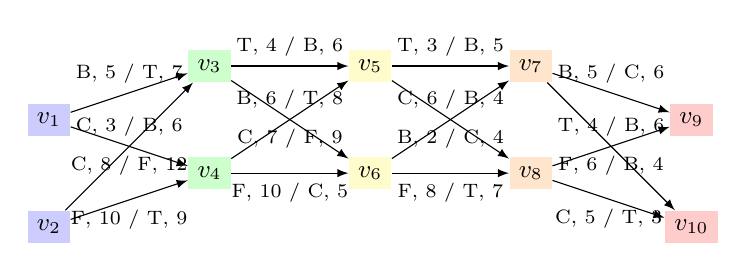
\begin{tikzpicture}[scale=0.68, every node/.style={font=\small}]
    % Nodes
    \node[fill=blue!20] (v1) at (0, 4) {$v_1$};
    \node[fill=blue!20] (v2) at (0, 2) {$v_2$};
    \node[fill=green!20] (v3) at (3, 5) {$v_3$};
    \node[fill=green!20] (v4) at (3, 3) {$v_4$};
    \node[fill=yellow!20] (v5) at (6, 5) {$v_5$};
    \node[fill=yellow!20] (v6) at (6, 3) {$v_6$};
    \node[fill=orange!20] (v7) at (9, 5) {$v_7$};
    \node[fill=orange!20] (v8) at (9, 3) {$v_8$};
    \node[fill=red!20] (v9) at (12, 4) {$v_9$};
    \node[fill=red!20] (v10) at (12, 2) {$v_{10}$};

    % Edges with multiple mediums
    \draw[-latex] (v1) -- (v3) node[midway, above, font=\scriptsize] {B, 5 / T, 7};
    \draw[-latex] (v1) -- (v4) node[midway, below, font=\scriptsize] {C, 8 / F, 12};
    \draw[-latex] (v2) -- (v3) node[midway, above, font=\scriptsize] {C, 3 / B, 6};
    \draw[-latex] (v2) -- (v4) node[midway, below, font=\scriptsize] {F, 10 / T, 9};
    \draw[-latex] (v3) -- (v5) node[midway, above, font=\scriptsize] {T, 4 / B, 6};
    \draw[-latex] (v3) -- (v6) node[midway, below, font=\scriptsize] {C, 7 / F, 9};
    \draw[-latex] (v4) -- (v5) node[midway, above, font=\scriptsize] {B, 6 / T, 8};
    \draw[-latex] (v4) -- (v6) node[midway, below, font=\scriptsize] {F, 10 / C, 5};
    \draw[-latex] (v5) -- (v7) node[midway, above, font=\scriptsize] {T, 3 / B, 5};
    \draw[-latex] (v5) -- (v8) node[midway, below, font=\scriptsize] {B, 2 / C, 4};
    \draw[-latex] (v6) -- (v7) node[midway, above, font=\scriptsize] {C, 6 / B, 4};
    \draw[-latex] (v6) -- (v8) node[midway, below, font=\scriptsize] {F, 8 / T, 7};
    \draw[-latex] (v7) -- (v9) node[midway, above, font=\scriptsize] {B, 5 / C, 6};
    \draw[-latex] (v7) -- (v10) node[midway, above, font=\scriptsize] {T, 4 / B, 6};
    \draw[-latex] (v8) -- (v10) node[midway, below, font=\scriptsize] {C, 5 / T, 3};
    \draw[-latex] (v8) -- (v9) node[midway, below, font=\scriptsize] {F, 6 / B, 4};
\end{tikzpicture}
\caption{Road network with categories $C_1$ to $C_5$.}
\label{fig:example_graph}
\end{figure}

\begin{theorem}
The Algorithm \ref{Alg:optimal_journey} always terminates within a finite number of steps for any valid input graph $\mathcal{G}$. 
\end{theorem}
\begin{proof}
Let $|\mathcal{V}|$ be the number of PoIs and $|\mathcal{E}|$ be the number of edges in the input graph $\mathcal{G}$. Each PoI and edge from the input is processed once to construct $\mathcal{G}$, which takes $\mathcal{O}(|\mathcal{V}| + |\mathcal{E})$. If the graph is disconnected, edges are added between disconnected components. Let $\mathcal{C}_1, \mathcal{C}_2, \dots, \mathcal{C}_p$ denote the $p$ connected components of the graph. At most $p-1$ edges are added to connect these components, which is a finite operation. For each category $\mathcal{C} = \{C_1, C_2, \dots, C_k\}$, the algorithm iterates through all pairs of PoIs $i \in C_{c-1}, j \in C_c$. Let $|C_c|$ denote the number of PoIs in category $C_c$. Then the pairwise iterations across all categories take at most $\sum_{c=2}^k |C_{c-1}| \cdot |C_c| \leq |\mathcal{V}|^2$. Next, the shortest path computations are performed using Dijkstra’s algorithm \cite{dijkstra2022note} with complexity \(O(|\mathcal{E}| \cdot \log|\mathcal{V}|)\) for each source-target pair. Since there are \(|C_{c-1}| \cdot |C_c|\) such pairs, the total complexity for path computations is $ \mathcal{O}(|\mathcal{V}|^2 \cdot |\mathcal{E}| \cdot \log|\mathcal{V}|)$. The dynamic programming (DP) updates for costs and paths iterate over \(|C_c|\) PoIs per category, taking \(O(|\mathcal{V}| \cdot |\mathcal{C}|)\). Each algorithm stage involves a finite number of operations, and no infinite loops are possible because the graph and categories are finite. Thus, the algorithm terminates.
\end{proof}

\begin{theorem}
If the input graph $\mathcal{G}$ is connected (or made connected by the algorithm), the Algorithm \ref{Alg:optimal_journey} guarantees a feasible journey from sources $v^{s}_i$ to destinations $v^{d}_i$. 
\end{theorem}

\begin{proof}
Let $\mathcal{G} = (\mathcal{V}, \mathcal{E}, W)$ be the input graph. If $\mathcal{G}$ is not connected, the algorithm identifies connected components $\mathcal{C}_1, \mathcal{C}_2, \dots, \mathcal{C}_p$, which ensures $\bigcup_{i=1}^p \mathcal{C}_i = \mathcal{V}, \quad \mathcal{C}_i \cap \mathcal{C}_j = \emptyset \text{ for } i \neq j $. For each pair of disconnected components, an edge is added between a PoI $v_i \in \mathcal{C}_i\) and $v_j \in \mathcal{C}_j$. At most $p-1$ edges are added, ensuring that the graph becomes connected i.e., $\text{diameter}(\mathcal{G}) < \infty$. Next, for each source $v^{s}_i$, the algorithm computes the shortest path to every PoI in $C_1$ using Dijkstra's algorithm, which guarantees $\exists \text{path}(v^{s}_i, v_j) \quad \forall v_j \in C_1 $. By mathematical induction on the categories, we assume a path exists from $v^{s}_i$ to any $v_j \in C_{c-1}$. The algorithm computes the shortest path from $v_j$ to all $v_k \in C_c$, ensuring $\exists \text{path}(v^{s}_i, v_k) \quad \forall v_k \in C_c$. In the final PoI to destinations, the algorithm computes the shortest path from the last PoI in $C_k$ to each destination $v^{d}_i$, ensuring $\exists \text{path}(v^{s}_i, v^{d}_i) \quad \forall v^{d}_i \in \mathcal{V}$. Thus, a feasible journey exists for all source-destination pairs.
\end{proof}

\begin{theorem}
The Algorithm \ref{Alg:optimal_journey} computes a journey with the minimum total cost between sources $v^{s}_i$ and destinations $v^{d}_i$. 
\end{theorem}

\begin{proof}
Let $\mathcal{G} = (\mathcal{V}, \mathcal{E}, W)$ be the input graph and $DP[c][j]$ represent the minimum cost to reach PoI $j \in C_c$ from any source $v^{s}_i$. The recurrence relation for $DP$ is $DP[c][j] = \min_{i \in C_{c-1}} \big(DP[c-1][i] + \text{ShortestPathCost}(i, j)\big)$. For the base case $(c=1)$, $DP[1][j] = \sum_{i \in v^{s}_i} \text{ShortestPathCost}(i, j)$. Now, applying mathematical induction on categories, we assume $DP[c-1][i]$ stores the minimum cost to reach $i \in C_{c-1}$. The Algorithm \ref{Alg:optimal_journey} computes the cost for $j \in C_c$ by evaluating all transitions $i \to j$ and taking the minimum, ensuring optimality $DP[c][j] = \min_{i \in C_{c-1}} (DP[c-1][i] + W(i, j))$. By mathematical induction, $DP[c][j]$ stores the minimum cost for all paths ending at $j \in C_c$. Now, for final transitions to the destinations, for each destination $v^{d}_i$, the total cost is$    \text{TotalCost} = \sum_{j \in C_k} DP[k][j] + \sum_{j \in v^{d}_i} W(j, v^{d}_i)$. Since all pairwise costs are minimized in the DP updates, the final cost is also minimized. Thus, the algorithm computes the globally optimal journey.
\end{proof}

\section{Experimental Evaluation} \label{Sec:EE}
In this section, we describe the experimental evaluation of the proposed solution approach. Initially, we start by describing the datasets used in our experiments. 


\subsection{\textbf{Dataset Description}}
We evaluate our proposed approach with two different real-world datasets. First, the networks of Switzerland, which are previously used by Sauer et al. \cite{potthoff2022efficient, sauer2020efficient, bez2024fast}, and the second is the road network of Helsinki\footnote{\url{https://welcome.hel.fi/}} city of Finland. The public transit network for Switzerland and Finland are collected from GTFS feed\footnote{\url{https://gtfs.geops.ch/}}. The Switzerland network covers the timetable of two business days, and the road networks were obtained from OpenStreetMap\footnote{\url{https://download.geofabrik.de/}}. The Finland dataset includes travel time and distance between all SYKE (Finnish Environment Institute), calculated for walking, cycling, public transport, and car travel \cite{tenkanen2020longitudinal}. This data covers two times of day: midday and rush hour. In Switzerland network we merged seven different feeds `Bus', `Train', `Ferry', `Funicular', `Gondola', `Subway' and `Tram' into a single transport network. We categorize the PoIs into ten distinct categories `Train Station', `Public Square', `City Center', `Bridge', `School', `Park', `Bus Stop', `Airport', `Healthcare Facility' and `Hotel'. Further, we compute the travel cost for each medium of transport using (Travel Cost = Base Fare + (Cost per minute * Travel Time) + (Cost per meter * Travel Distance)) the information provided in Table \ref{tab:transport_fares}. In the pre-processing steps, we eliminate the PoI pair from the Switzerland network in which the source and destination PoI are the same. In the case of the Finland dataset, there are complete transport road networks for the city of Helsinki. However, in our problem context, we have taken a small portion of the road networks that contain $1100$ unique PoIs. One point to be highlighted is the fares given in Table \ref{tab:transport_fares}, \ref{tab:transport_costs_helsinki} are the approximate fares we assumed for our problem context. An overview of the networks is given in the Table \ref{Table:Dataset}.

\begin{table}[h!]
\scriptsize
\caption{Base Fare, Cost per Meter, and Cost per Minute for Different Transport Modes in Switzerland}
\centering
\begin{tabular}{|c|c|c|c|}
\hline
\textbf{Transport Medium} & \makecell{\textbf{Base Fare} \\ \textbf{(CHF)}} & \makecell{\textbf{Cost per Meter} \\ \textbf{(CHF)}} & \makecell{\textbf{Cost per Minute} \\ \textbf{(CHF)}} \\ \hline
Bus & 2.50 - 4.00 & 0.01 - 0.03 & 0.05 - 0.10 \\ \hline
Tram & 2.50 - 4.00 & 0.01 - 0.03 & 0.05 - 0.10 \\ \hline
Train & $\sim$5.00 & 0.03 - 0.05 & 0.10 - 0.15 \\ \hline
Ferry & 5.00 - 10.00 & 0.05 - 0.10 & 0.15 - 0.25 \\ \hline
Funicular & 1.30 - 5.00 & 0.02 - 0.04 & 0.10 - 0.15 \\ \hline
Gondola & 5.00 - 15.00 & 0.05 - 0.15 & 0.20 - 0.50 \\ \hline
Subway & 2.50 - 4.00 & 0.01 - 0.03 & 0.05 - 0.10 \\ \hline
\end{tabular}
\label{tab:transport_fares}
\end{table}

\begin{table}[h!]
\scriptsize
\caption{Base Fare, Cost per Meter, and Cost per Minute for Different Transport Modes in Helsinki, Finland}
\centering
\begin{tabular}{|l|c|c|c|}
\hline
\textbf{Transport Medium} & \makecell{\textbf{Base Fare} \\ \textbf{(EUR)}} & \makecell{\textbf{Cost per Meter} \\ \textbf{(EUR)}} & \makecell{\textbf{Cost per Minute} \\ \textbf{(EUR)}} \\ \hline
% Walking & 0.00 & 0.00 & 0.00 \\ \hline
Bike & 0.00 - 5.00 & 0.00 - 0.10 & 0.05 - 0.10 \\ \hline
Public Transport & 3.20 & 0.03 - 0.05 & 0.05 - 0.10 \\ \hline
Private Car (Taxi) & 5.90 & 0.01 - 0.05 & 0.74 \\ \hline
\end{tabular}
\label{tab:transport_costs_helsinki}
\end{table}

%Further, we calculate the distance of the PoIs from the transfer graph of Switzerland and compute travel cost using travel distance and time \cite{mathisen2006relationship}. 

\begin{table}[h!]
	% \scriptsize
	\caption{Dataset Description}
	\label{Table:Dataset}
	\centering
	\begin{tabular}{ccc}
	\hline
	\textbf{Attributes} & \textbf{Switzerland} & \textbf{Finland}  \\ \hline
	Stops  & 44557  &    1100 \\ 
	Routes & 168294  & 4840000\\
	Vertices & 1310  & 1100 \\
	Edges & 11370  &  604950\\
	\hline\\
	\end{tabular}
\end{table}

% \paragraph{\textbf{Key Parameter}}
% We vary the number of agents $(|\mathcal{U}|)$ by $5,10,20,50,100$ to show the effectiveness and efficiency of the proposed solution approach. We also vary the number of PoIs in the intermediate category to show the scalability of the proposed and baseline methods. We present all our experimental results considering the $10$ intermediate category. However, we have experimented for a different number of categories, say $5,10,20$.

% % \vspace{-0.25in}
% \begin{table}[h!]
% \caption{\label{Key-parameters} Key Parameters}
% \vspace{-0.15 in}
% \begin{center}
%     \begin{tabular}{ | p{2cm}| p{5cm}|}
%     \hline
%     Parameter & Values  \\ \hline
%     $|\mathcal{U}|$ & $5,10,20,50,100$   \\ \hline
%     $PoI$ & $5,10,15,20$   \\ \hline
%     $Category$ & $5, 10, 20$   \\ \hline
%     \end{tabular}
% \end{center}
% \end{table}
\subsection{\textbf{Environment and Key Parameter Setup}} \label{Sec:Env_Setup} The proposed and baseline methods are implemented in Python using the Jupyter Notebook Platform. All the experiments are conducted in a Ubuntu-operated desktop system with 64 GB RAM and an Xeon(R) 3.5 GHz processor. Next, we vary the number of agents $(|\mathcal{U}|)$ by $5,10,20,50,100$ to show the effectiveness and efficiency of the proposed solution approach. We also vary the number of PoIs in the intermediate category to show the scalability of the proposed and baseline methods. However, we have experimented for a different number of categories, say $5,10,20$. We present all our experimental results considering the $10$ as the default number of the intermediate category. We have experimented with all our codes three times, and the average results are reported. 

\subsection{\textbf{Baseline Methodologies}} \label{Sec:Baseline}
\paragraph{\textbf{Random PoI and Random Medium (RPRM)}}
In this approach, from source to destination via intermediate categories of PoI, the PoIs are selected randomly, and the transport medium between two PoIs is chosen randomly.

\paragraph{\textbf{Random PoI and Cheapest Medium (RPCM)}}
This approach selects PoIs randomly from source to destination via intermediate categories of PoI; however, consider the cheapest transport medium to visit one PoI to others.

\paragraph{\textbf{Nearest Neighbor PoI and Cheapest Medium (NNCM)}}
This approach considered the nearest PoI in the first category of PoIs from the source using the cheapest transport medium, and from onwards, it selects one PoI from each category, considering the same till the destination.

\subsection{\textbf{Goals of our Experiments}} \label{Sec:Research_Questions}
The following research questions (RQ) are our focus in this study.
\begin{itemize}
\item \textbf{RQ1}: Varying number of agents, how do the travel cost and computational time change?
\item \textbf{RQ2}: Varying number of agents, how does the usage of transport medium change?
\item \textbf{RQ3}: Varying number of PoI in each category, how do the computational time and transport medium change?
\end{itemize}

\subsection{\textbf{Experimental Results and Discussions}}
In this section, we will address the research questions posed in Section \ref{Sec:Research_Questions} and discuss the experimental results.
%% \vspace{-0.25cm}
\begin{figure*}[h!]
\centering
\begin{tabular}{cccc}
\includegraphics[scale=0.18]{Plots/Agent5.pdf} 
& \includegraphics[scale=0.18]{Plots/Agent10.pdf} 
& \includegraphics[scale=0.18]{Plots/Agent20.pdf}
& \includegraphics[scale=0.18]{Plots/Agent50.pdf} \\
\tiny{(a) $|\mathcal{U}| = 5$} &  \tiny{(b) $|\mathcal{U}| = 10$} & \tiny{(c) $|\mathcal{U}| = 20$} & \tiny{(d) $|\mathcal{U}| = 50$} \\
\includegraphics[scale=0.18]{Plots/Agent100.pdf} &
\includegraphics[scale=0.18]{Plots/FA_Usage_5.pdf} &
\includegraphics[scale=0.18]{Plots/FA_Usage_10.pdf} &
\includegraphics[scale=0.18]{Plots/FA_Usage_20.pdf} \\
\tiny{(e) $|\mathcal{U}| = 100$} & \tiny{(f) $|\mathcal{U}| = 5$} &  \tiny{(g) $|\mathcal{U}| = 10$} & \tiny{(h) $|\mathcal{U}| = 20$} \\
\includegraphics[scale=0.18]{Plots/FA_Usage_50.pdf} &
\includegraphics[scale=0.18]{Plots/FA_Usage_100.pdf} &
\includegraphics[scale=0.18]{Plots/FA_Varying_PoI_Cost.pdf} &
\includegraphics[scale=0.18]{Plots/FA_Varying_POI_Time1.pdf} \\
\tiny{(i) $|\mathcal{U}| = 50$} & \tiny{(j) $|\mathcal{U}| = 100$}  & \tiny{(k) No. of PoI Vs. Cost}  & \tiny{$(\ell)$No. of PoI Vs. Time}
\end{tabular}
\caption{ Varying $|\mathcal{U}|$ Vs. Usage of transport medium in Switzerland $(a,b,c,d,e)$ and in Finland $(f,g,h,i,j)$, Varying No. of PoI Vs. Cost (k) and  Varying No. of PoI Vs. Time $(\ell)$  for Switzerland dataset}
\label{Fig:1Plot}
\end{figure*}

\begin{figure*}[h!]
\centering
\begin{tabular}{cccc}
 \includegraphics[scale=0.18]{Plots/AgentVsCost.pdf} &
\includegraphics[scale=0.18]{Plots/AgentVsTime.pdf} &
\includegraphics[scale=0.18]{Plots/FA_AgentVs_Cost.pdf} &
\includegraphics[scale=0.18]{Plots/FA_AgentVs_Time.pdf}    \\
\tiny{(a)  Varying $|\mathcal{U}|$ Vs. Cost}  & \tiny{(b) Varying $|\mathcal{U}|$ Vs. Time} & \tiny{(c)  Varying $|\mathcal{U}|$ Vs. Cost}  & \tiny{(d) Varying $|\mathcal{U}|$ Vs. Time} \\
\end{tabular}
\caption{ Varying $|\mathcal{U}|$ in Switzerland $(a,b)$ and in Finland $(c,d)$}
\label{Fig:2Plot}
\end{figure*}
\subsubsection{\textbf{No. of Agents Vs. Travel Cost}}
In this work, we vary the number of agents by $5, 10, 20, 50$, and $100$ to evaluate the transport cost via the different mediums of the journey. In Figure \ref{Fig:2Plot}$(a)$, \ref{Fig:2Plot}$(c)$, with the increase in the number of agents, the travel costs also increase, and from source to the first category and the last category to the destinations contribute significant costs in total travel while increasing the number of agents. In the Finland dataset, the proposed `OJPA' approach provides less cost than the baseline methods like `NNCM', `RPCM', and `RPRM', and among the baseline methods, the `NNCM' provides less cost and the `RPRM' provides maximum cost. This happens because the `NNCM' always picks the nearest PoI and cheapest medium of journey, and on the other hand, the `RPRM' always picks a PoI and medium of journey randomly. In the case of the Switzerland dataset, similar observations were found as those in Finland, as reported in Figure \ref{Fig:2Plot}$(c)$. For example, in the Finland dataset, when the number of agents is $5$, the travel costs for `OJPA,' `NNCM,' `RPCM,' and `RPRM' are $42.75$ \euro, ~$160.765$\euro, ~$237.5$ \euro ~and ~$244.6$ \euro, respectively. When the number of agents is $100$, the travel costs for `OJPA', `NNCM', `RPCM',  and `RPRM' are $745.75$ \euro, ~$2569.23$ \euro, ~$4156.25$ \euro, and ~$4156.25$ \euro, respectively. Now, in the Switzerland datasets, when the number of agents varies from $5$ to $100$, the travel costs for `OJPA', `NNCM', `RPCM',  and `RPRM' are $30701.25$ CHF,	$68861.25$ CHF,	$308353.75$ CHF, and $204588.75$ CHF to $15005950$ CHF,	$75782150$ CHF,	$103046875$ CHF, and $70440000$ CHF, respectively. The reason behind providing a huge cost in the Switzerland dataset is that, in most cases, no direct paths are available in the road network. In most cases, direct paths between two PoIs are available in the Finland dataset. For this reason, the proposed `OJPA,' as well as all the baseline methods, provides fewer costs than the Switzerland dataset.

\subsubsection{\textbf{No. of Agents Vs. Time}}
To determine the computational time required, we vary the number of agents and observe the run time is proportional to a varying number of agents. We have compared our proposed approach with baseline methods like `NNCM,' `RPCM,' and `RPRM' and among them `NNCM' takes more time compared to the baselines like `RPCM,' and `RPRM' as well as the `OJPA' approach. This happens because `NNCM', finds the nearest PoI from one category to the PoIs from another. It is also considered the cheapest medium of the journey, which leads to huge computational time. However, the `RPCM' and `RPRM' both methods use randomization for the selection of PoIs from one category to another, and this leads to very less runtime, and it is negligible compared to the other methods. These observations are consistent with both Switzerland as well as Finland datasets, as shown in Figure \ref{Fig:2Plot}$(b)$ and \ref{Fig:2Plot}$(d)$, respectively. For example, in the Switzerland dataset, when we vary agents from $5$ to $100$, the runtime for `OJPA', `NNCM', `RPCM', and `RPRM' varies from $24,25,2,2$ to $546,605,58,53$ in seconds, respectively. 

\subsubsection{\textbf{No. of Agents Vs. Medium Usage}}
The usage of travel medium varies when the number of agents varies. Figure \ref{Fig:1Plot}$(a)$ to \ref{Fig:1Plot}$(j)$ shows the varying number of agents, how the usage of different transport mediums varies. In the Switzerland dataset, we have considered different mediums of the journey, i.e., `bus (BS)', `ferry (FR)', `gondola (GD)', `subway (SW)', `tram (TM)', `train (TN)'. Now, with the increase in the number of agents, the usage of different mediums increases, and only `bus', `ferry', `gondola', and `tram' are used as the travel medium for all the proposed and baseline methods. In all the cases, `Bus' is the most used medium while `gondola' is the least used medium of journey. In figure \ref{Fig:1Plot}$(a,b,c,d,e)$, we have reported the average usage of the travel mediums, and from the figure, it is clear that the Unknown (UN) medium has the highest usage. This happens in the dataset because the road network is not well connected, and to build a connected graph, we used additional edges. During the journey, most of the agents chose the edges in their optimal paths. In the `OJPA' and `NNCM', the usage of different mediums is almost the same, while the `RPCM' and `RPRM' have very far different usage of mediums due to the randomization nature. The Finland dataset consists of three journey modes: public transport (PT), private car (PC), and bike, and they are used very frequently. Public transport and private cars are the most used medium, as reported in Figure \ref{Fig:1Plot}$(f,g,h,i,j)$. We have observed that with the increase in the number of agents, the usage of private cars as a medium increases and public transport usage decreases. These observations are consistent with the Switzerland dataset.

\subsubsection{\textbf{Additional Discussion}}
Additionally, we have experimented with varying numbers of PoIs in each category to check the computational time requirements and usage of different mediums of the journey. We fixed the number of agents as $100$ and varied the number of PoIs in each category by $5, 10, 15,$, and $20$, and the experimental results are reported in Figure \ref{Fig:1Plot}$(k, \ell)$. We have observed that the computational time increases rapidly with the increased number of agents. Now, in the case of medium usage, minor changes happen in the case of the `OJPA' and `NNCM' approaches. However, major changes in usage occur in the `RPCM', and `RPRM'. We have also varied the number of intermediate categories by $5,10,20$ and observed that with an increasing number of categories, the computational cost increases rapidly. One point needs to be noted in the Switzerland and Finland datasets: we have considered an equal number of PoIs in each category, including the source and destination categories for all our experiments as default settings.


\section{Concluding Remarks} \label{Sec:CFD}
In this paper, we have studied the GTP query problem in the presence of multiple transport mediums for commuting. To the best of our knowledge, this is the first study on GTP Query Problem in this direction. We show that as the number of categories of PoIs increases, the problem becomes intractable. We have proposed a dynamic programming-based approach, and the proposed methodology has been analyzed to understand its time and space requirements. We conduct a large number of experiments with publicly available benchmark datasets. From the experiments, we have observed that the proposed solution approach leads to a much better quality solution compared to many baseline methods. Now, this study can be extended in the following directions. As the objective of our study is to minimize the aggregated cost of the group, it may happen that the individual cost for some agents may be too high compared to others. Hence, tackling the fairness issue in our problem context is an important direction for future research. 

\bibliographystyle{IEEEtran}
\bibliography{Paper}



\end{document}

\end{document}